\documentclass{standalone}

\usepackage{tikz}
\usetikzlibrary{arrows,decorations.pathmorphing,positioning,fit,petri}
\usetikzlibrary{calc,intersections,through,backgrounds,graphs}
\usetikzlibrary{patterns,decorations.pathreplacing}

\begin{document}

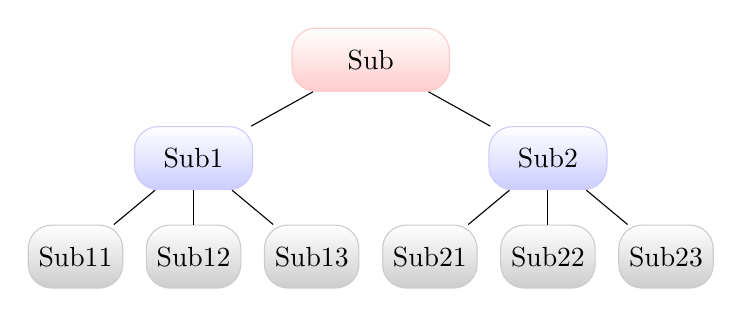
\begin{tikzpicture}
	% Styles
	[
	sub/.style={rectangle, rounded corners=3mm, minimum size=8mm, minimum width=1.2cm, draw=black!20, top color=white, bottom color=black!20},
	mid/.style={rectangle, rounded corners=3mm, minimum size=8mm, minimum width=1.5cm, draw=blue!20, top color=white, bottom color=blue!20},
	top/.style={rectangle, rounded corners=3mm, minimum size=8mm, minimum width=2cm, draw=red!20, top color=white, bottom color=red!20}
	]
                      
	% Nodes
	\node at (3.75,2.5)	(sub)	[top] {Sub};
	\node at (1.5,1.25)	(sub1)	[mid] {Sub1};
	\node at (6,1.25)	(sub2)	[mid] {Sub2};
	\node at (0,0)		(sub11)	[sub] {Sub11};
	\node at (1.5,0)	(sub12)	[sub] {Sub12};
	\node at (3,0)		(sub13)	[sub] {Sub13};
	\node at (4.5,0)	(sub21)	[sub] {Sub21};
	\node at (6,0)		(sub22)	[sub] {Sub22};
	\node at (7.5,0)	(sub23)	[sub] {Sub23};
	
	% Connections
	\graph[use existing nodes] {
		sub -- sub1;
		sub -- sub2;
		sub1 -- sub11;
		sub1 -- sub12;
		sub1 -- sub13;
		sub2 -- sub21;
		sub2 -- sub22;
		sub2 -- sub23;
	};

\end{tikzpicture}

\end{document}